\documentclass[10pt,conference,compsocconf]{IEEEtran}

\usepackage[utf8]{inputenc}
\usepackage{hyperref}
\usepackage{graphicx}	% For figure environment
\usepackage{subfig}

\begin{document}
\title{Machine Learning Course - Project 1}

\author{
  Quentin Laville, Valentin Moullet, Joël M. Fonseca\\
  \textit{Department of Computer and Communication Sciences, EPFL, Switzerland}
}

\maketitle

%%%%%%%%%%%%%%%%%%%%%%%%%%%%%%%%%%%%%%%%%%%%%%
\section{Introduction}

The whole process described here concerns the first project of the CS-433 Machine Learning class. The goal is to apply various machine learning models on a dataset provided by the CERN, generated by the Large Hadron Collider, in order to distinguish experiences resulting in background from Higgs boson decay.

%%%%%%%%%%%%%%%%%%%%%%%%%%%%%%%%%%%%%%%%%%%%%%%
\section{The Data}

\subsection{Provided}

Two datasets are given: a training and test set. The train set contains more than $N_1 = 250k$ experiences with outcomes (either a 'b' for background, and 's' for signal $-$ i.e., a Higgs boson decay). The test set contains more than $N_2 = 500k$ experiences without the outcome. Each sample was described by a row of $D = 30$ features.

\subsection{Pre-processing}

\subsubsection{Standardization}

We standardize both the training and the test sets using the training mean and variance.

\subsubsection{Dataset split}

After analyzing the data sets, one can notice that only one feature is categorical: $PRI\_jet\_num$ takes value in $[0,3]$. Moreover, some features seems to match a pattern following this $jet$ number. Thus, data points having $jet=0$ miss a lot of values, the same when $jet=1$ but in a lesser proportion and when $jet=2$ or $jet=3$, the values for the features are almost complete (as well as being quite correlated). After this exploration, we decided to train the data points that have different $jet$ numbers separately, as they look like different in nature.

\subsubsection{Missing values}

As experiences could not always give relevant data, missing values ($-999.0$) were filled with a $NaN$ values. As we have seen above, some features don't make sense anymore for some $jet$ values, hence they are removed. For the others, the $NaN$ values are replaced by the median of the corresponding column.

\subsubsection{Features engineering}

In order to get more from the data we received, we decided to add some columns (features) computed from the basic features. We did that in two different ways:
\begin{itemize}
\item Addition of inverse logarithm for positive-only features: for each feature that was always positive (except for $-999.0$), we computed the inverse logarithm of it and added a new column with those new values. The goal of this was to get more information out of the few features we started with (30), and intuitively it makes our model penalizing less the big differences between numbers in those features. In other words, we try to find some hidden relationships by transforming other features.
\item Polynomial expansion: for each feature $x$, we added columns representing $x^2$, $x^3$, ... until the degree we are using (grid search with cross validation is done to find the best degree for each model).
\end{itemize}

\begin{table*}[htbp]
  \centering
  \begin{tabular}[c]{|l||c|c|}
    \hline
    Model name&Accuracy mean&Accuracy std\\
    \hline
    Least squares&0.8105&0.0454\\
    Ridge regression&0.8447&0.0050\\
    Gradient descent&0.8245&0.0053\\
    Stochastic gradient descent&0.6888&0.1439\\
    Logistic regression&0.8137&0.0262\\
    Regularized logistic regression&0.8186&0.0224\\
    \hline
  \end{tabular}
  \caption{Accuracy results for $PRI\_jet\_number=0$ split.}
  \label{tab:jet0}
\end{table*}

%%%%%%%%%%%%%%%%%%%%%%%%%%%%%%%%%%%%%%%%%%%%%%%%
\section{Machine Learning Models and Methods}

\subsection{Models}

The following models were used throughout the project:

\begin{enumerate}
\item Gradient descent ($\gamma$, $iterations$)
\item Stochastic gradient descent ($\gamma$, $iterations$)
\item Least square with a polynomial basis ($degree$)
\item Ridge regression with a polynomial basis ($degree$, $\lambda$)
\item Logistic ($degree$, $iterations$, $\gamma$)
\item Regularized logistic regression ($degree$, $iteration$, $\gamma$, $\lambda$)
\end{enumerate}

All the parameters inside the parentheses are exhaustively tested by grid search. 

\begin{enumerate}
\item $iterations \in \{50, 100, ... , 250\}$
\item $degree \in \{1, 2, ... , 15\}$
\item $\gamma \in \{0.05, 0.1, ... , 1.0\}$
\item $\lambda \in \{1\mathrm{e}{-5} ... , 1\mathrm{e}{-2}\}$
\end{enumerate}

Note that the last parameter is computed in logarithmic space.


\subsection{Cross validation}
To train and test the different models, the 10-fold cross validation is used. This technique consists in splitting the data set in 10 size-equivalent bins. Then each bin is selected as the test bin, one after the other, and the 9 remaining ones are used to train the model. When the model is ready, you can check its validity against the test bin. This is helpful to avoid the overfitting of a particular model over the training set.

\subsection{Accuracy estimation}

To compute accuracy, we simply compared the resulting $y_{train}$ and the true $y$ and computed the percentage of matching values. By the 10-fold cross validation, the final accuracy was computed by doing the mean of each $y_{train}$ obtained for each iteration. On top of that, we also computed the variance in order to see that the accuracy is indeed stable among the different folds.

\subsection{Best Model}

After using all models created with all related parameters with grid search, ridge regression gives the best results. It's quite surprising, as we expect the logistic models to be better, the problem being a classification one (tell if a sample results in a Higgs boson decay or not). Note that we didn't use balancing because we saw that it wasn't helping the overall accuracy against the test set, which could mean that the proportion is more or less the same in the training set than in the test set; we still think that balancing in general is important.

%%%%%%%%%%%%%%%%%%%%%%%%%%%%%%%%%%%%%%%%%%%%%%%%%
\section{Results}

The Table~\ref{tab:jet0} and Figure~\ref{fig:plots} are all computed using only the $jet$ number 0. Similar plots can be done for the other $jet$ number values. Nevertheless, we obtained the best results with ridge regression each time. 

The two figures tell us that the polynomial expansion gives pretty good results, especially for the Ridge regression. Indeed, we see that having a high degree allows us to perform better, but only until degree 12 (which is already quite high); the lambda should be quite low in order to have good results for Ridge regression. For the logistic regression figure, we see that changing the gamma does not affect a lot the performance, and having a degree bigger than 2 makes the performance worst.

As explained above, we can now see from Table~\ref{tab:jet0} that indeed logistic performs below ridge regression, which is quite unexpected. 

Finally, let's point that stochastic gradient descent is poorly represented here, mostly because of the batch size of 1. Other batch sizes were tested during the process, all of them giving better results.

\begin{figure}
\centering
\subfloat[Ridge Regression]{
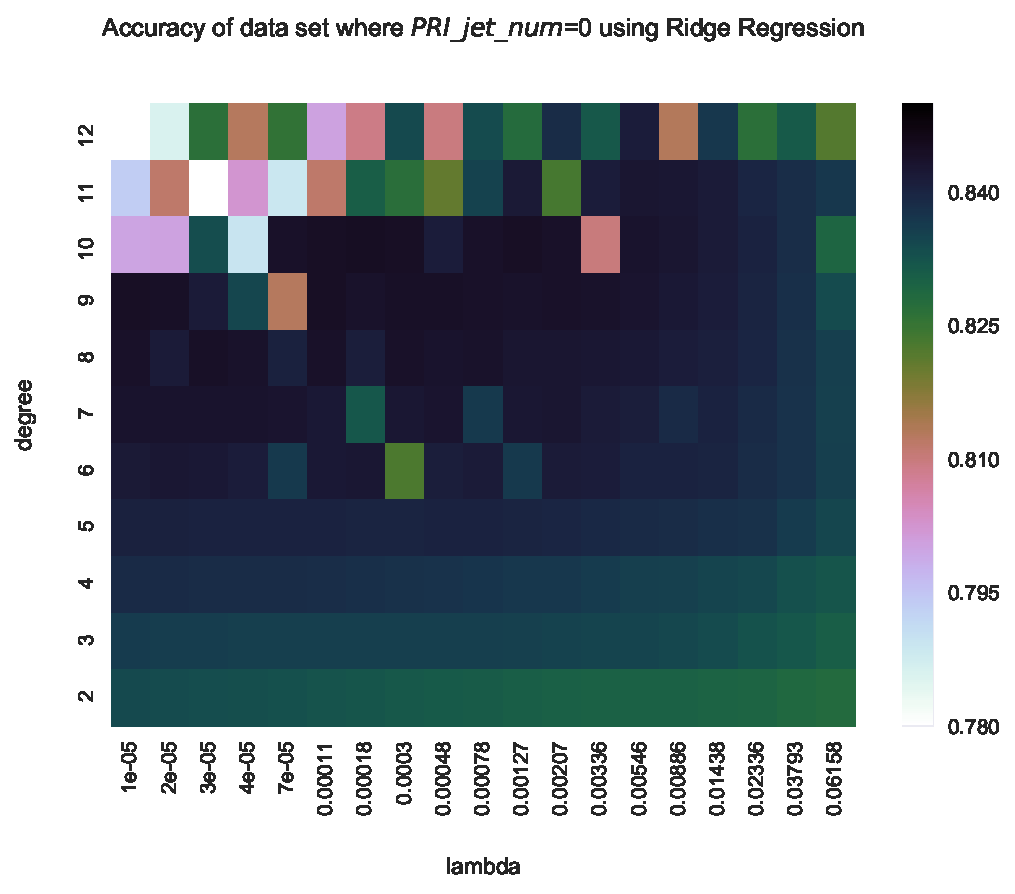
\includegraphics[width=85mm]{figures/0_ridge_regression}
}
\newline
\subfloat[Logistic Regression ]{
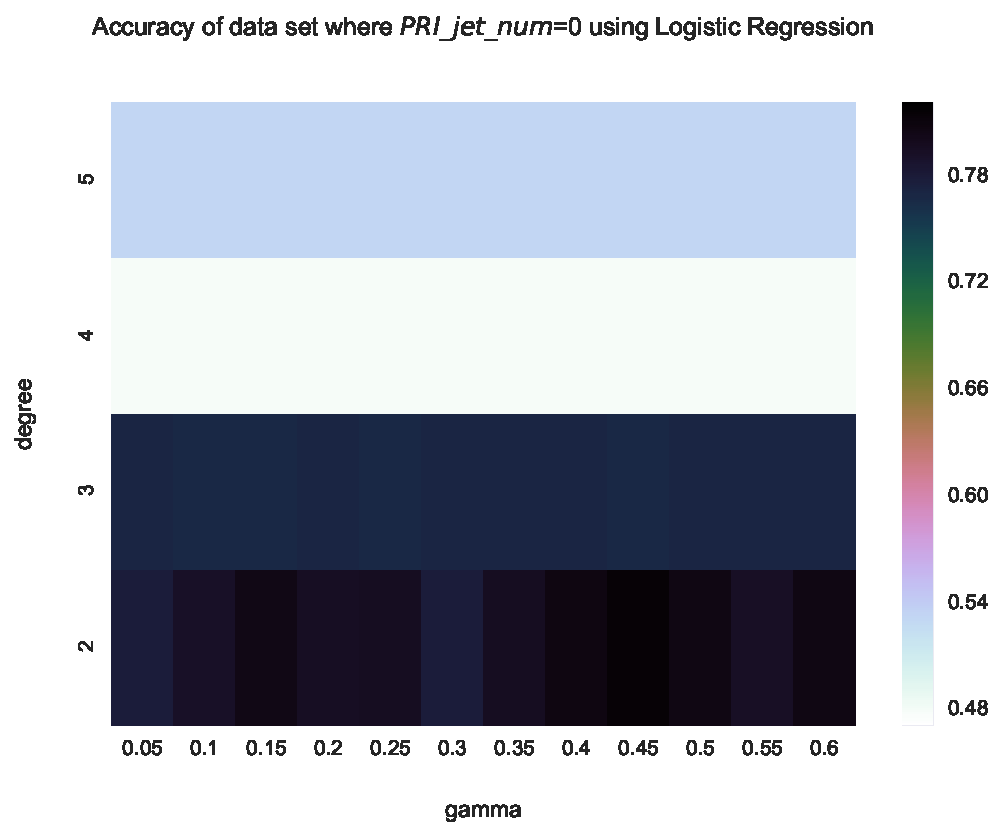
\includegraphics[width=85mm]{figures/0_logistic_regression}
}
\caption{Grid search for different models for $PRI\_jet\_number=0$ split.}
\label{fig:plots}
\end{figure}

\end{document}
